\begin{tikzpicture}[overlay, remember picture]
    \node[anchor=north west, rotate=0, gray, font=\tiny, text width=\paperwidth] at (current page.south west)  [xshift=0, yshift=0.75cm] {
    [1] L. Amico et al., Entanglement in Many-Body Systems, Reviews of Modern Physics 80, no. 2 (2008)
    };
\end{tikzpicture}


\only<1,2>{

Peres-Horodecki criterion of being separable (sufficient):
\vspace{-2mm}
\begin{equation*}
    \rho_{AB}^{T_B} \geq 0.
\end{equation*}
\vspace{-5mm}


% \phantom{42}

\begin{minipage}{0.55\textwidth}
    Necessary for:
    \begin{itemize}
        \iitem{two qubits}
        \iitem{two harmonic oscillator modes}
    \end{itemize}
\end{minipage}
\hfill
\begin{minipage}{0.4\textwidth}
\begin{figure}[h]
    \centering
    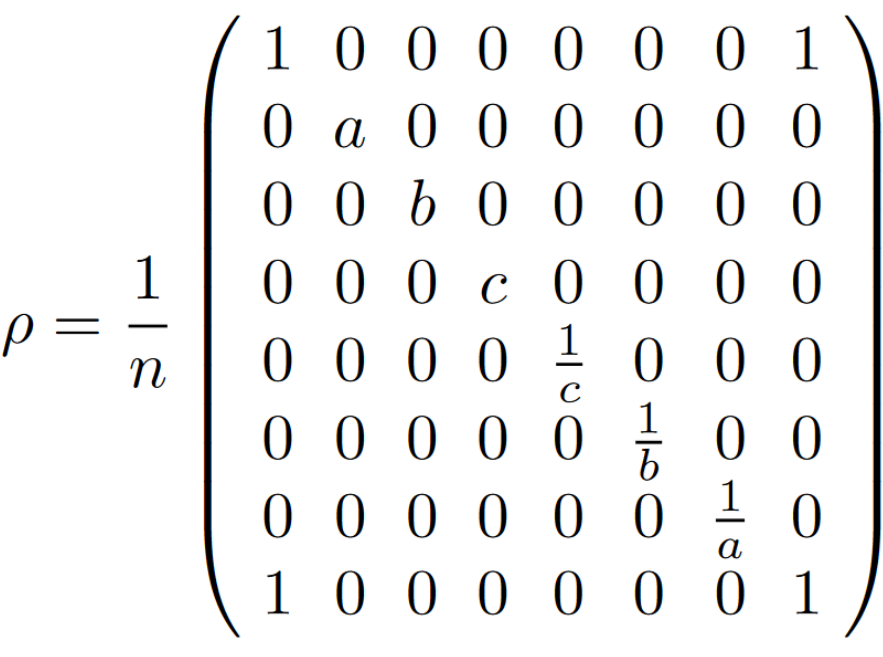
\includegraphics[width=\textwidth]{imgs/ppp.png}
    %\caption{}
    %\label{fig:}
\end{figure}

\end{minipage}



\phantom{42}

\onslide<2>{

Measure of entanglement: \textit{the logarithmic negativity}
\vspace{-3mm}
\begin{equation*}
    E_N = \log_2 (2 N_{AB} + 1), \vspace{-3mm}
\end{equation*}
with $N_{AB}$ is the absolute sum of the negative eigenvalues of $\rho_{AB}^{T_B}$.

}
}